\section{INTEGRATION STRATEGY}
\subsection{Entry Criteria} 
Before the integration testing can begin, both the RASD and the DD must be completed. Furthermore at least the 80\% of the lines of the code of all components must have been tested with a Unit Test. We strongly suggest the Junit testing framework for Unit Testing.
\subsection{Elements to be Integrated} 
As we have described in the DD, the main components of the system are:
\begin{itemize}
\item Web Client GUI
\item Mobile Client GUI
\item Driver Client GUI
\item Service Manager 
\item HTTP Server
\item Request Handler
\item REST Parser
\item DBMS
\end{itemize}

In turn, the Service Manager is composed of:
\begin{itemize}
\item Car Manager
\item Trip Manager
\item User Manager
\item Position Manager
\item Fee Manager
\end{itemize}
\noindent
For a further description of the components refer to the Design Document. 
\newline 
Of course, because before the Service Manager can be integrated with other components, the components that compose it have to be integrated.


\subsection{Integration Testing Strategy} 

We have chosen for the Integration Testing a \textbf{bottom up} approach. This means that the integration will regard first the low-level components. For this type of testing, because we start from the low level components, we will need some \textbf{drivers}. These are temporary modules that simulate the behaviour of the higher level components and do the calls of the functions of lower level components. \newline
That reason why we have chosen the bottom-up approach are:

\begin{itemize}
\item The lowest level component of our system is the DBMS, impletemented with MySQL 5.6. MySQL is a well-known software component that is available on the market. So the DBMS is ready to use and is a robust starting point for the Integration Testing. Starting from this we can begin to integrate the component of Backend of our system, that essentialy is the Service Manager component. 
\item The low level components that compose the Backend of our service are the biggest part of our system and all the other components depends on them. Because of this importance of the low level components, the best choice is to start from them and, when it's sure that they work well together, integrate the other components.
\end{itemize}  

When the integration testing regards the Service Manager, the bottom up approach will be mixed with the \textbf{functional testing} approach. With functional testing, not the entire components are tested, but only some functionalities of them. In our case, when the components that compose the Service Manager will be tested together with the Service, only some functionalities of the Service Manager will be tested, that are the ones that call the specific subcomponent that is being tested.
\subsection{Sequence of Component/Function Integration} 
\subsubsection{Software Integration Sequence} For each subsystem, identify the sequence in which the software components will be integrated within the subsystem; relate this sequence to any product features that are being built up
\newline
\todo{i componenti che vengono aggiunti a livello più alto devono essere dei driver, non i componenti stessi}
Because we have chosen a bottom up approach, the first components to be tested are the low level ones, so the ones that compose the Service Manager. After we have completed the integration for the subcomponents of the Service Manager, we will integrate the components that are directly interfaced with that subsystem, that are the Car Manager and the Request Manager. At the end, we will integrate the remaining front-end components, that are the Web Client and the Mobile Client.
At each step of the integration, a driver for the new component to be integrated has to be constructed. When the integration testing regarding that component stops, the driver is replaced with the actual component.
\paragraph{User Manager}
\todo{vanno messe le didascalie giuste alle immagini}
The first component that will be tested is the User Manager, because he has a relation with the DBMS, that is a component ready to use, as we mentioned in the previous paragraph. In particular it has to manipulate data about the users and their account.
So first the User Manager is integrated with the DBMS:

\begin{figure}[H]	
	\centering
	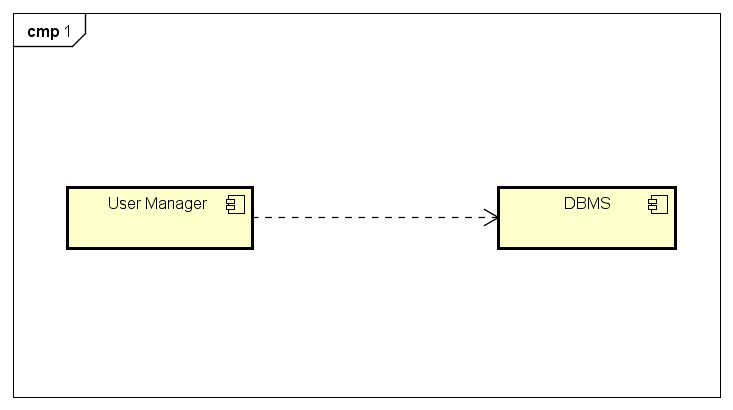
\includegraphics[width=\textwidth]{img/UserMan_DBMS_int}
	\caption{Component Diagram}
\end{figure}
\noindent
When the two components are proved to work well together, the functions of the Service Manager regarding the use of the User Manager are added: \todo{del service manager vengono integrate solo un po' di funzionalità alla volta, quindi l'approccio è un mix tra Bottom Up e Functional Testing}

\begin{figure}[H]	
	\centering
	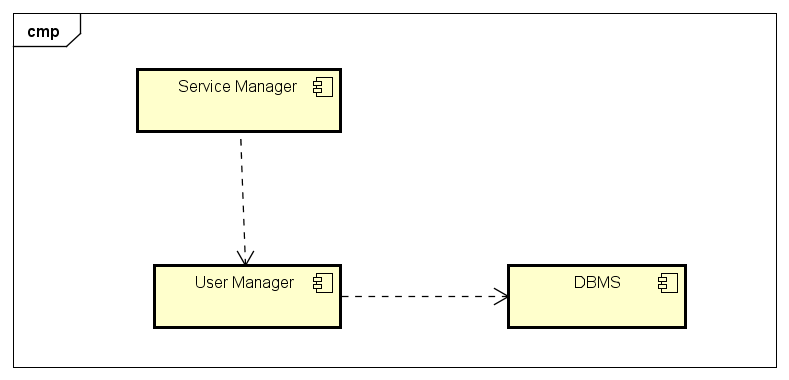
\includegraphics[width=\textwidth]{img/UserMan_SrvMan_int}
	\caption{Component Diagram}
\end{figure}
\paragraph{Reservation Manager}
The second component that will be tested is the Reservation Manager, because he too has a relation with the DBMS. In particular, it has to manipulate data regarding the cars:

\begin{figure}[H]	
	\centering
	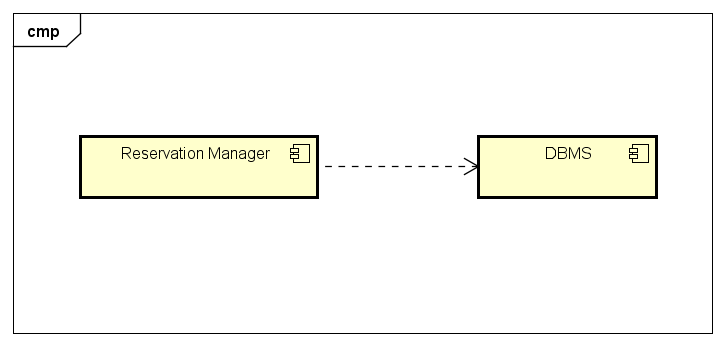
\includegraphics[width=\textwidth]{img/ResMan_DBMS_int}
	\caption{Component Diagram}
\end{figure}

After the Reservation Manager is well integrated with the DBMS, we integrate the two components together with the specific functionalities of the Service Manager

\begin{figure}[H]	
	\centering
	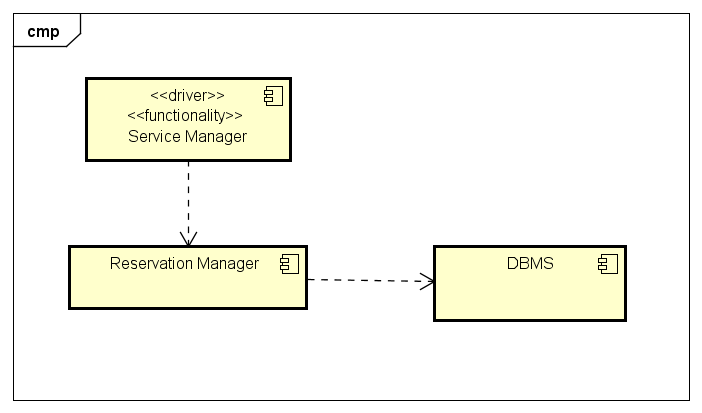
\includegraphics[width=\textwidth]{img/ResMan_SrvMan_int}
	\caption{Component Diagram}
\end{figure}
\paragraph{Fee Manager}
The Fee Manager have to be tested first with the payment system. Because it would be hard and expensive using a real payment system, a stub simulating its functionalities is used:

\begin{figure}[H]	
	\centering
	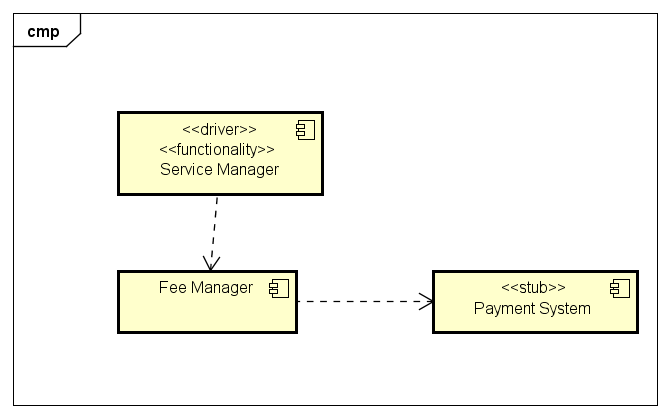
\includegraphics[width=\textwidth]{img/FeeMan_PaySys_int}
	\caption{Component Diagram}
\end{figure}
After that, the Fee Manager will be integrated with the proper functionalities of the Service Manager:

\begin{figure}[H]	
	\centering
	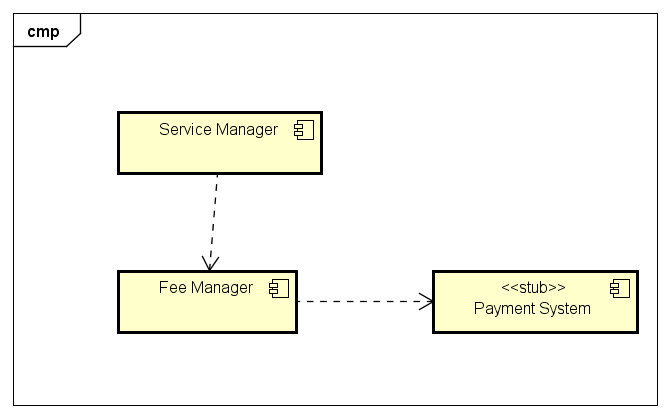
\includegraphics[width=\textwidth]{img/FeeMan_SrvMan_int}
	\caption{Component Diagram}
\end{figure}
\paragraph{Position Manager}
The Position Manager have to be tested first with the GPS software. Because the development team is already provided with the GPS software, we don't need the use of a stub but we can integrate the real software:

\begin{figure}[H]	
	\centering
	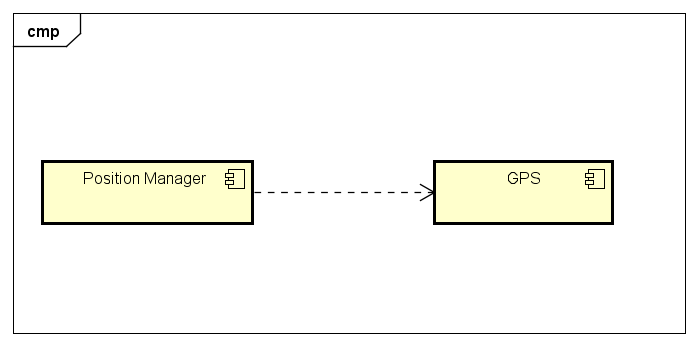
\includegraphics[width=\textwidth]{img/PosMan_GPS_int}
	\caption{Component Diagram}
\end{figure}
Then the components are integrated with the functionalities of the Service Manager:

\begin{figure}[H]	
	\centering
	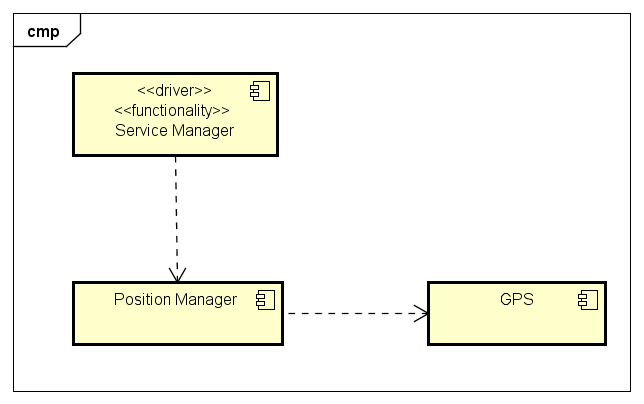
\includegraphics[width=\textwidth]{img/PosMan_SrvMan_int}
	\caption{Component Diagram}
\end{figure}

\paragraph{Car Manager}
The Car Manager is interfaced only with the Service Manager, so it is tested only with that component:

\begin{figure}[H]	
	\centering
	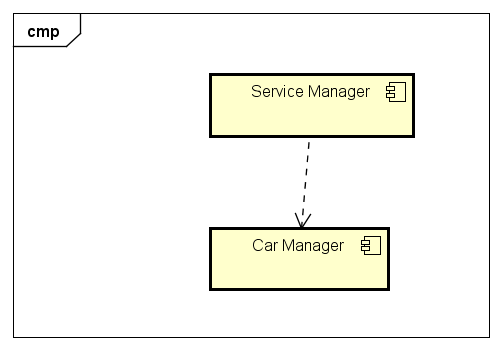
\includegraphics[width=\textwidth]{img/CarMan_SrvMan_int}
	\caption{Component Diagram}
\end{figure}

\paragraph{Service Manager}
After the integration tests on the subcomponents of the System Manager are completed, the Service Manager is ready to be integrated with higher level components. The testing of the subcomponents of the Service Manager ends here because those subcomponents implement functionalities that are independent with each other and so is sufficient to test them singularly together with the Service Manager and the external components they need.
\newline
So, after the completion of the test on the Service Manager, this component will have to be tested with the Request Handler and the Car Manager, that are the components directly interfaced with the Service Manager.
First we choose to integrate the Request Handler, because it is the most critical component:


\begin{figure}[H]	
	\centering
	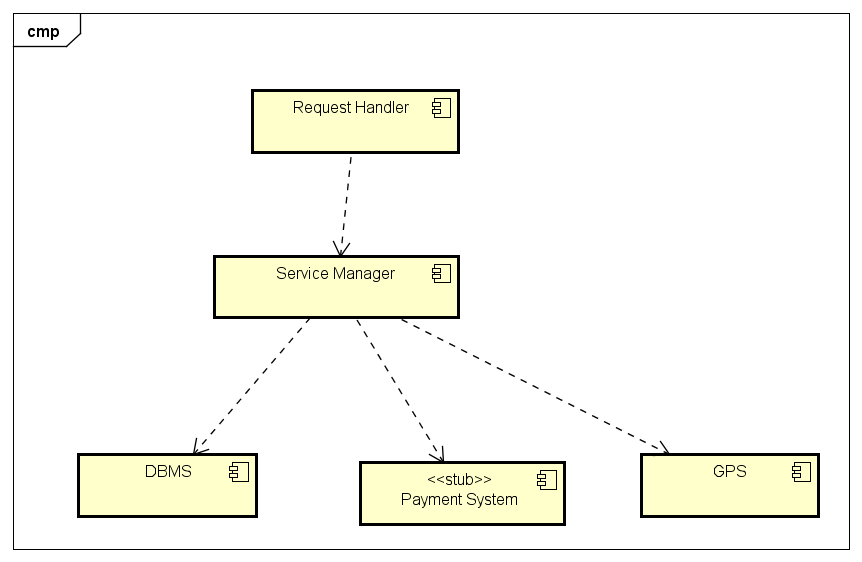
\includegraphics[width=\textwidth]{img/SrvMan_ReqHan_int}
	\caption{Component Diagram}
\end{figure}

Then, the Service Manager will be integrated with the OnBoard Device:


\begin{figure}[H]	
	\centering
	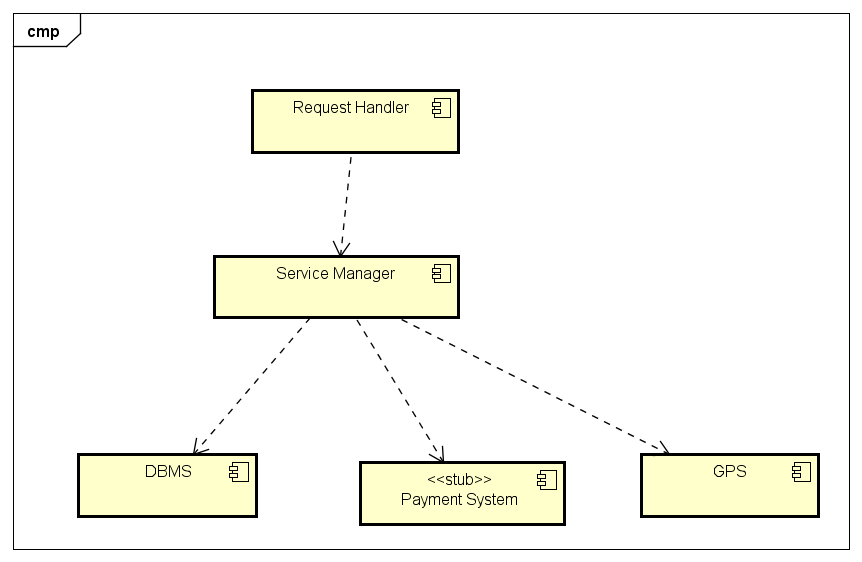
\includegraphics[width=\textwidth]{img/SrvMan_ReqHan_int}
	\caption{Component Diagram}
\end{figure}

\paragraph{Request Handler}
After the integration of the Request Handler and OnBoard Device, we can integrate the resulting subsystem with the HTTP Server. In particular the focus is on the interaction between the Request Handler and the HTTP Server:
\begin{figure}[H]	
	\centering
	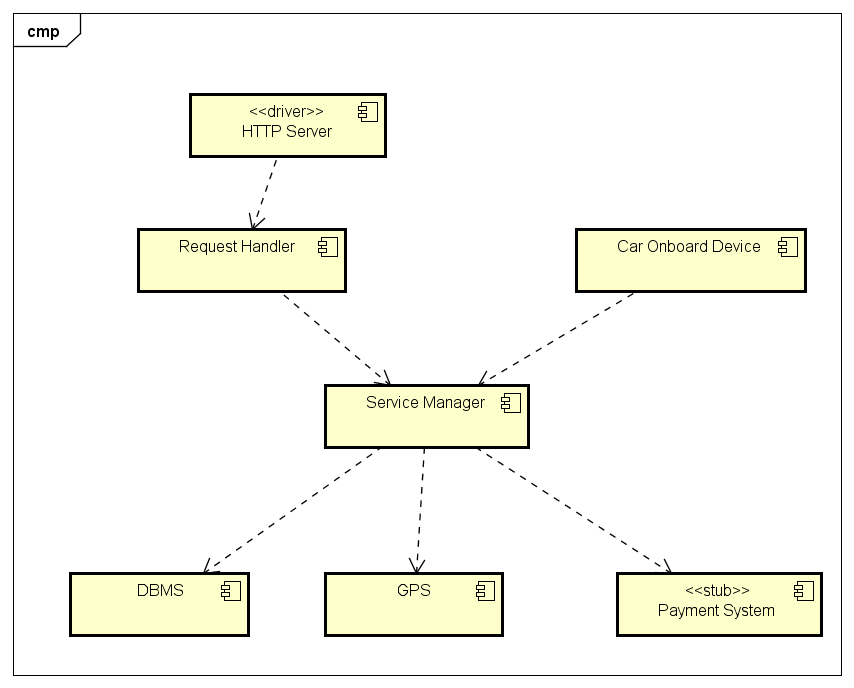
\includegraphics[width=\textwidth]{img/ReqHan_HTTP_int}
	\caption{Component Diagram}
\end{figure}

\paragraph{HTTP Server}
In the end, when the HTTP Server driver is substituted by the real component, the remaining two frontend components are integrated: the Mobile Client and the Web Client. The order in which this two components are chosen doesn't matter:
\begin{figure}[H]	
	\centering
	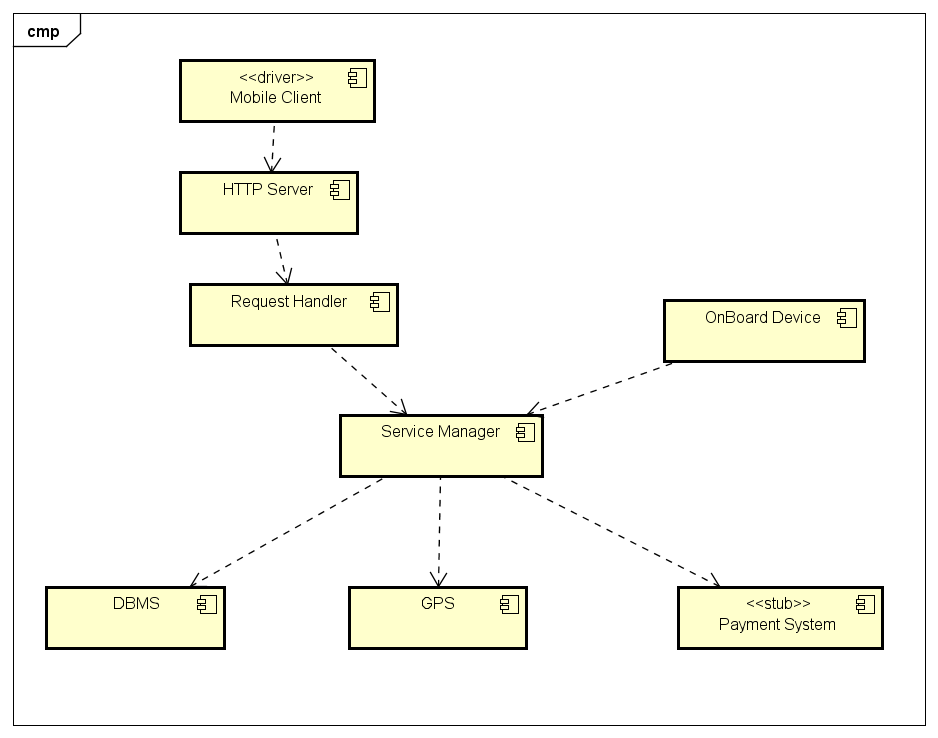
\includegraphics[width=\textwidth]{img/HTTP_MobCli_int}
	\caption{Component Diagram}
\end{figure}

\begin{figure}[H]	
	\centering
	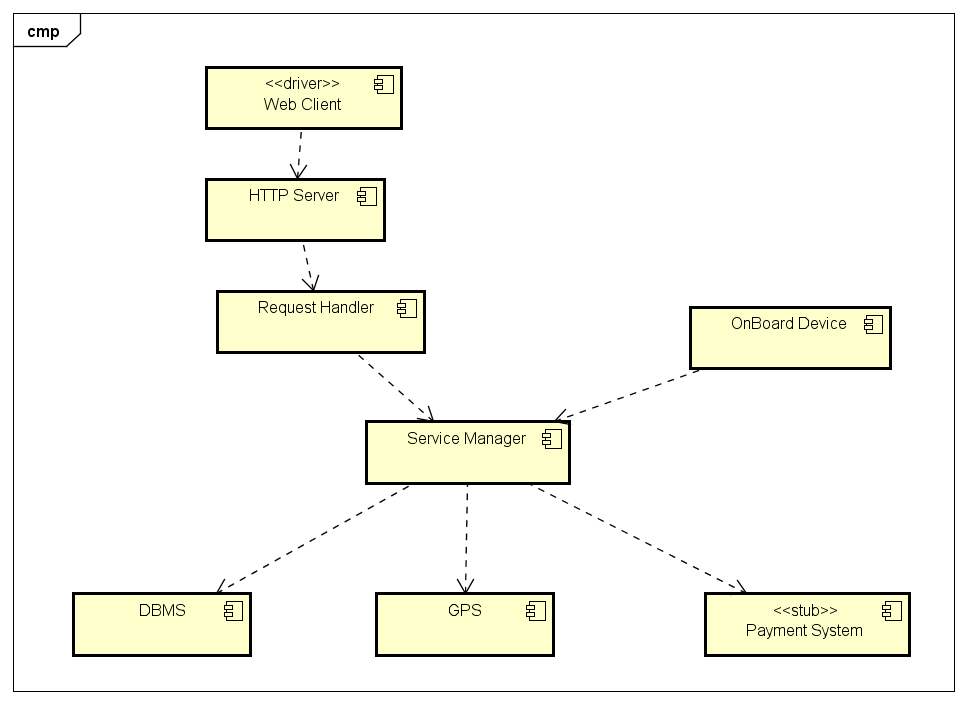
\includegraphics[width=\textwidth]{img/HTTP_WebCli_int}
	\caption{Component Diagram}
\end{figure}

After these two integration tests, the all components of the system can be tested together.

\subsubsection{Subsystem Integration Sequence} Identify the order in which subsystems will be integrated;  if you have a single subsystem, 2.4.1 and 2.4.2 have to be merged in a single section





